% Chapter Template

\chapter{Superconducting Qubit Theory} % Main chapter title

\label{Chapter3} % Change X to a consecutive number; for referencing this chapter elsewhere, use \ref{ChapterX}

%----------------------------------------------------------------------------------------
%	SECTION 1
%----------------------------------------------------------------------------------------
\section{Classical LC oscillator}

%------------ FILL THE LC OSCILLATOR FIGURE -----------
\begin{figure}
\centering
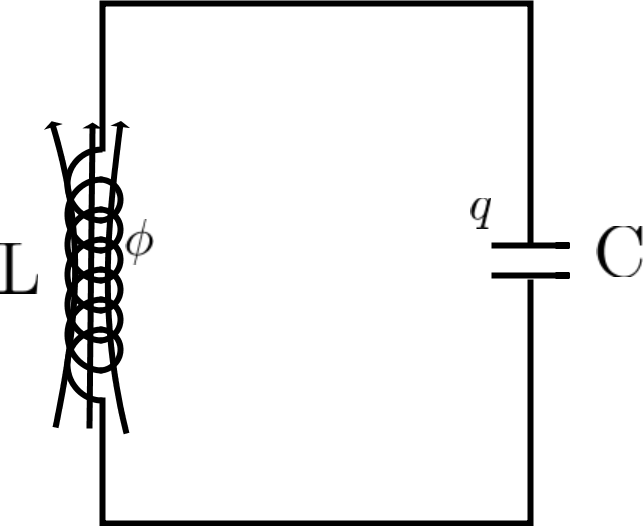
\includegraphics[width=150pt]{Figures/LC_oscillator}
\decoRule
\caption[LC oscillator]{LC oscillator circuit}
\label{fig:LC oscillator}
\end{figure}

The LC oscillator, shown in Fig.\ref{fig:LC oscillator}, when treated classically has a charge $q$ on the capacitor, and a flux $\phi$ in the inductor. The flux is related to the charge via the inductance as $\phi=L\dfrac{dq}{dt}$. The Hamiltonian for this circuit is
\begin{equation}
\mathcal{H}=\frac{q^2}{2C}+\frac{\phi^2}{2L}
\end{equation}

\section{Quantum Electrical Circuits}

\subsection{Quantum LC oscillator}

Observe that the 2 variables involved in the LC oscillator, $q$ and $\phi=L\dfrac{dq}{dt}$, are similar in form to the position and momentum operators in quantum mechanics, $\hat{x}$ and $\hat{p}=-j\hbar\dfrac{\partial}{\partial x}$. Even the Hamiltonian is of the same form.\parencite{Devoret1995}
\begin{equation}
\hat{\mathcal{H}}=\frac{\hat{p}^2}{2m}+\frac{m\omega^2\hat{x}^2}{2}
\end{equation}
Because of this, we can treat this circuit like the simple harmonic oscillator and introduce the annihilation and creation operators to define $\hat{q}$, $\hat{\phi}$ and Hamiltonian operators as
\begin{subequations}
\begin{align}
\hat{\phi}&=\frac{1}{j}\sqrt{\frac{\hbar}{2Z_0}}(a-a^\dag)\\
\hat{q}&=\sqrt{\frac{\hbar Z_0}{2}}(a+a^\dag)\\
\hat{\mathcal{H}}&=\frac{\hbar\omega_0}{2}(a^\dag a+aa^\dag)=\hbar\omega_0\left(a^\dag a + \frac{1}{2}\right)
\label{eqn:harmonic hamiltonian}
\end{align}
\end{subequations}
where
\begin{align*}
[\hat{\phi},\hat{q}]=-j\hbar&&
\omega_0=\frac{1}{\sqrt{LC}}&&
Z_0=\sqrt{\frac{L}{C}}
\end{align*}
$\omega_0$ and $C$ in the LC oscillator is analogous to $\omega$ and $m$ in the harmonic oscillator.

We can write the wave-functions of the energy eigenstates of the LC oscillator as
\begin{equation}
\bra{x}\ket{0}=\psi_0=\left(\frac{C\omega_0}{\pi\hbar}\right)^\frac{1}{4}e^{-\left(\frac{C\omega_0}{2\hbar}\right)x^2}
\end{equation}
This solution can be obtained using $a\ket{0}=0$

The rest of the eigenstates can be obtained by using the creation operator $a^\dag$ since
\begin{equation}
a^\dag\ket{n}=\sqrt{n+1}\ket{n+1}
\end{equation}
which gives
\begin{equation}
\ket{n}=\frac{(a^\dag)^n}{\sqrt{n!}}\ket{0}
\end{equation}
The energy corresponding to these states are
\begin{equation}
E_n=\left(n+\frac{1}{2}\right)\hbar\omega_0
\end{equation}
The general solution to the Schr\"{o}dinger equation $\hat{\mathcal{H}}\ket{\psi}=E\ket{\psi}$ is
\begin{equation}
\ket{\psi}=\sum_nc_n\ket{n}
\end{equation}
The first few energy levels along with the corresponding wavefunctions are shown in Fig.\ref{fig:harmonic oscillator}.

\begin{figure}
\centering
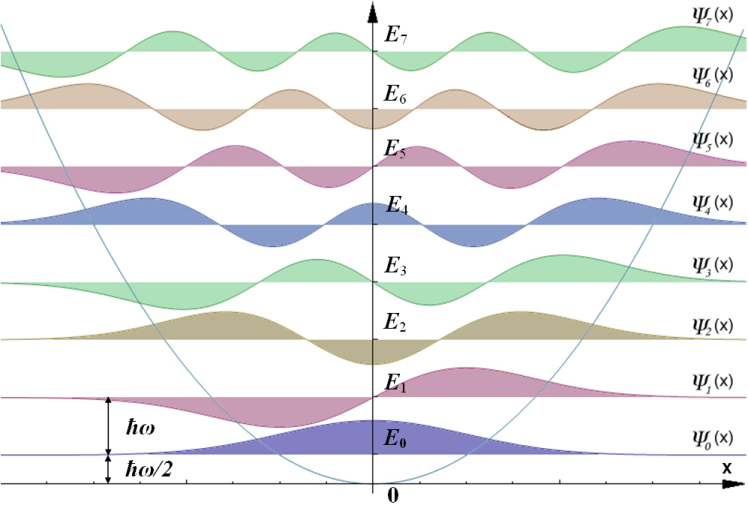
\includegraphics[width=\linewidth]{Figures/harmonic_oscillator}
\decoRule
\caption[Harmonic Oscillator Energy Levels]{The harmonic oscillator potential showing the Energy Levels $E_1,E_2,\ldots$ along with the corresponding wavefunctions $\psi_1,\psi_2,\ldots$. Replacing the position coordinate here with charge would give us the Energy levels for an LC oscillator.Taken from \\© \href{https://pl.wikipedia.org/wiki/Wikipedysta:Tomasz59}{User:Tomasz59} / \href{http://commons.wikimedia.org/}{Wikimedia Commons} / \href{http://creativecommons.org/licenses/by-sa/3.0/}{CC-BY-SA-3.0}}
\label{fig:harmonic oscillator}
\end{figure}

Coherent states of a harmonic oscillator are defined as the eigenstates of the amplitude operator, or annhilation operator $a$, such that
\begin{equation}
a\ket{\alpha} = \alpha\ket{\alpha}
\end{equation}
where $\alpha = |\alpha|e^{j\varphi}$ is a complex number and corresponds to the complex wave amplitude in classical optics. Thus coherent states are wave-like states of the electromagnetic oscillator is a complex number \cite{Glauber1963}.

The coherent state $\ket{\alpha}$ can be represented in terms of the number states $\ket{n}$ as
\begin{equation}
\ket{\alpha} = \sum_{n=0}^\infty \frac{\alpha^n}{\sqrt{n!}}e^{-|\alpha|^2/2}\ket{n}
\label{eqn:glauber expansion}
\end{equation}

\subsection{Nonlinear Harmonic Oscillator}

Note that the energy levels in the Simple Harmonic Oscillator (SHO) or the LC oscillator are equispaced. This means that if we supply a photon of energy $\hbar\omega_0$ to the LC oscillator, we can change the state from any $\ket{n}$ to $\ket{n+1}$, and all photons emitted due to the transition from $\ket{n}$ to $\ket{n-1}$ will have the same energy.

A Nonlinear Harmonic Oscillator is one where the energy levels do not increase linearly. We can create a nonlinear oscillator by adding a perturbation to the Hamiltonian. The new Hamiltonian will be of the form
\begin{equation}
\hat{\mathcal{H}}=\frac{q^2}{2C}+\frac{\phi^2}{2L} +\mathcal{H}'
\end{equation}
where $H'$ is the perturbation term.
The energy levels for this new Hamiltonian can be written in terms of the unperturbed Hamiltonian using perturbation theory as
\begin{equation}
E_n=E_n^{(0)}+\expval{\mathcal{H}'}{n^{(0)}}+\sum_{k\neq n}\frac{\left|\mel{k^{(0)}}{\mathcal{H}'}{n^{(0)}}\right|^2}{E_n^{(0)}-E_k^{(0)}}+\ldots
\end{equation}
where,\\
$E_n$ is the new energy for the $n$th eigenstate,\\
$E_n^{(0)}$ is the energy for the $n$th eigenstate of the unperturbed Hamiltonian,\\
$\expval{\mathcal{H}'}{n^{(0)}}$ is the first order correction to the energy and\\
$\sum_{k\neq n}\frac{\left|\mel{k^{(0)}}{\mathcal{H}'}{n^{(0)}}\right|^2}{E_n^{(0)}-E_k^{(0)}}$ is the second order correction to the energy.

If the perturbation $\mathcal{H}'$ is not a constant (i.e $\mathcal{H}'(n)\neq \mathcal{H}'(m)$ where $n\neq m$), then we can access only the ground state and the first exited state with one frequency of photons. This is because if the particle is in the first excited state, and another photon of the same energy ($E_{10}=E_1-E_0$) is supplied to the system, it will not excite the particle further.

This means that we can selectively access only 2 states. If we can manipulate such a 2 level system and it's interactions, we have a qubit!

\section{The Josephson Junction}

The \JJ is the nonlinear element used in the described experiments due to it's negligible dissipation rate which is essential for working in the quantum regime.\\
The \JJ is made of 2 superconductors coupled by a weak link. In our case the junction is an S-I-S (Superconductor-Insulator-Superconductor) junction as shown in Fig.\ref{fig:SISJJ}.

\begin{figure}
\centering
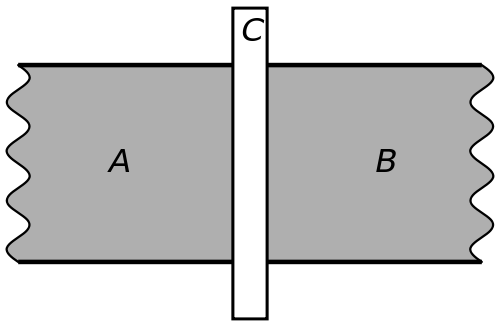
\includegraphics[width=\linewidth]{Figures/SISJJ}
\decoRule
\caption[Josephson Junction]{Simple geometric structure of a \JJ with A and B being superconducting regions and C being the thin insulating layer.}
\label{fig:SISJJ}
\end{figure}

Electrons in a normal metal behave like fermions. But at very low temperatures, they form cooper pairs that act like bosons. Nearly all the bosons will be at the lowest energy in exactly the same state \cite{Feynman1966}. This means that the superconductor will have a macroscopic wavefunction with a single homogeneous amplitude and phase.

In the \JJ, there are two superconductors, and so we can define 2 amplitudes and 2 phases corresponding to each superconductor.
\begin{align*}
\psi_1&=\sqrt{\rho_1}e^{j\theta_1}\\
\psi_2&=\sqrt{\rho_2}e^{j\theta_2}
\end{align*}
Then, the current and voltage characteristics are given by \cite{Harmans1997}
\begin{align}
I_s&=I_0\sin\delta
\label{eqn:JJ current}\\
V&=\frac{\Phi_0}{2\pi}\dot{\delta}
\label{eqn:JJ voltage}
\end{align}
where $\delta=\theta_2-\theta_1$ is the superconducting phase difference\footnote{This phase difference $\delta$ is the generalized phase difference $\delta=\Delta\theta-\displaystyle\dfrac{2\pi}{\Phi_0}\int A\cdot dl$} associated with the \JJ, $\Phi_0=h/2e$ is the flux quantum for a cooper pair and $I_0$ is the critical current of the junction.

We can view the \JJ as a nonlinear inductor and find the inductance simply by using $V=L_J\dfrac{dI_s}{dt}$ which gives $L_J$, the Josephson Inductance to be
\begin{equation}
L_J=\frac{\Phi_0}{2\pi}\frac{1}{I_0\cos\delta}
\end{equation}

In addition to this we can represent a real \JJ using the RCSJ model with a shunting capacitance ($C$) and resistance ($R$) along with the bare \JJ \cite{Harmans1997}. Then the current through the circuit is
\begin{equation}
I=I_s+\frac{V}{R}+C\frac{dV}{dt}
\end{equation}
by using \ref{eqn:JJ current} and \ref{eqn:JJ voltage} we get
\begin{equation}
C\left(\frac{\hbar}{2e}\right)^2\frac{d^2\delta}{dt^2}+\frac{1}{R}\left(\frac{\hbar}{2e}\right)^2\frac{d\delta}{dt}+\frac{\hbar}{2e}(I_0\sin\delta-I)=0
\end{equation}
We can see that this is the equation of motion of a particle moving along the $\delta$ coordinate with\\ an acceleration $\dfrac{d^2\delta}{dt^2}$,\\ drag force proportional to velocity $\dfrac{d\delta}{dt}$ and\\ force due to the gradient of the potential energy as the last term.\\
This leads to the "particle mass" given by
\begin{align}
M&=C\left(\frac{\hbar}{2e}\right)^2&&\text{"particle mass"}\\
U(I,\delta)&=-E_J\cos\delta-\left(\frac{\hbar}{2e}\right)I\delta&&\text{potential energy}
\end{align}
where $E_J$, the Josephson Energy is given by
\begin{equation}
E_J=\frac{\hbar}{2e}I_0=\frac{\Phi_0}{2\pi}I_0
\label{eqn:junction energy}
\end{equation}
The current $I$ is usually so small that we can ignore that term making the potential energy
\begin{equation}
U=-E_J\cos\delta
\label{eqn:JJ potential energy}
\end{equation}

The electrical energy stored in the capacitance is analogous to kinetic energy and can be calculated as
\begin{equation}
E_{kin}=\frac{1}{2}Mv^2=\frac{1}{2}C\left(\frac{\hbar}{2e}\right)^2\left(\frac{d\delta}{dt}\right)^2
\end{equation}

\section{The Cooper Pair Box}

The \CPB circuit is shown in Fig.\ref{fig:cooperpairbox}. It consists of a superconducting island capacitively coupled (with capacitance $C_g$) to a voltage source ($V_g$) connected to ground, and a \JJ connected to the ground. The \JJ can be represented by a capacitance ($C_j$) and the bare \JJ (represented by $E_J$) as shown in the figure.

\begin{figure}
\centering
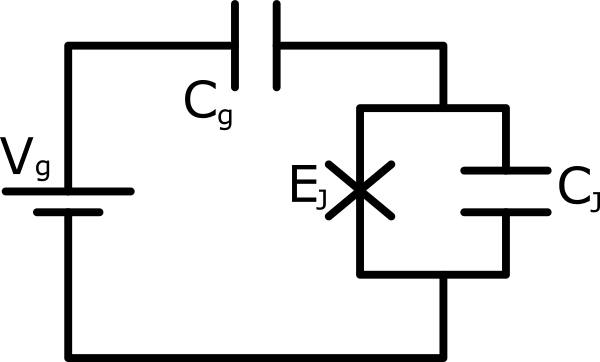
\includegraphics{Figures/CPB.png}
\decoRule
\caption[\CPB circuit]{The \CPB circuit with the \JJ represented as a bare \JJ with Josephson Energy $E_J$ and a capacitance $C_j$.}
\label{fig:cooperpairbox}
\end{figure}

The electrical energy of this circuit is the energy stored in the 2 capacitors, $C_g$ and $C_j$. If the total charge of the superconducting island is $-n|e|$, then the electrical energy ($\mathcal{H}_{el}$) is given by \cite{Schuster2007}
%---------------------------------------------------------
% Maybe you can show this in Appendix
%--------------------------------------------------------
\begin{equation}
\hat{\mathcal{H}_{el}}=4E_C(\hat{n}-n_g)^2
\end{equation}
where $\hat{n}\ket{n}=n\ket{n}$, $\ket{n}$ is the charge state with $n$ cooper pairs.\\
$E_C=e^2/2C_\Sigma=e^2/2(Cj+Cg)$ is the energy required to add one electron to the island and $n_g=C_gV_g/e$.\\
The energy levels are shown in Fig.\ref{fig:CPB EJ=0} for $E_J=0$. The \JJ would allow charge to tunnel through at $n_g=0.5,-0.5,1.5,-1.5\ldots$ in order to maintain the lowest energy.

\begin{figure}
\centering
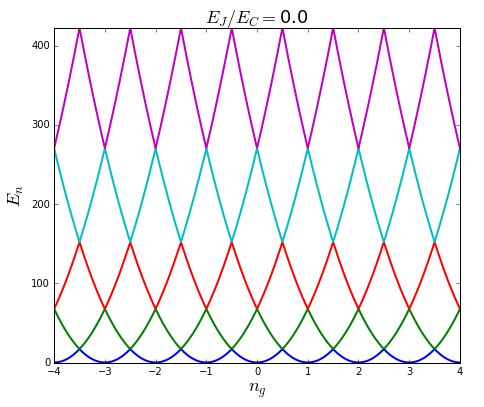
\includegraphics[width=300pt]{Figures/EjEc=0.png}
\decoRule
\caption[Energy Level for $E_J=0$]{Energy levels for $E_J=0$ or no tunneling. This figure was generated using \cite{Johansson2012}.}
\label{fig:CPB EJ=0}
\end{figure}

However, to calculate the complete Hamiltonian, we must also take into account the energy of the bare \JJ ($H_J$) which is given by.
\begin{equation}
\hat{\mathcal{H}_J}=-E_J\cos\hat{\delta}
\end{equation}
This is the tunnelling energy in the phase basis. To find the expression in the charge basis, we start with the commutation relation between charge and phase (See Appendix 1-A-2 from \cite{Cottet2002d}).
\begin{align}
\left[\hat{n},\hat{\delta}\right]&=-j
\label{eqn:commutation}
\end{align}
Using \ref{eqn:commutation} and the commutator identity \ref{eqn:comm identity}, we get
\begin{align}
\left[\hat{n},\hat{\delta}^m\right]&=\hat{\delta}^{m-1}\left[\hat{n},\hat{\delta}\right]+\hat{\delta}\left[\hat{n},\hat{\delta}^{m-1}\right]
\label{eqn:comm identity}\\
\end{align}
we can recursively use this relation to get
\begin{align}
\left[\hat{n},\hat{\delta}^m\right]&=-jm(\hat{\delta})^{m-1}\\
\hat{n}\hat{\delta}^m&=-jm\hat{\delta}^{m-1}+\hat{\delta}^m\hat{n}
\end{align}
The operator $\hat{n}e^{jp\hat{\delta}}$, where $p\in Z$, after expansion is
\begin{align}
\begin{split}
\hat{n}e^{jp\hat{\delta}}&=\hat{n}\sum_{m=0}^\infty \frac{( jp\hat{\delta})^m}{m!}=\sum_{m=0}^\infty \frac{(jp)^m\hat{n}\hat{\delta}^m}{m!}\\
&=\sum_{m=0}^\infty \frac{(jp)^m\hat{n}(\hat{\delta})^m}{m!}\\
&=\sum_{m=0}^\infty \frac{(jp)^m(-jm\hat{\delta}^{m-1}+\hat{\delta}^m\hat{n})}{m!}\\
&=\sum_{m=0}^\infty \frac{(jp)^m(-jm\hat{\delta}^{m-1})}{m!}+\sum_{m=0}^\infty \frac{(jp\hat{\delta})^m\hat{n}}{m!}\\
&=p\sum_{m=1}^\infty \frac{(jp\hat{\delta})^{m-1}}{(m-1)!}+\sum_{m=0}^\infty \frac{(jp\hat{\delta})^m\hat{n}}{m!}
\end{split}\\
\hat{n}e^{jp\hat{\delta}}&=pe^{jp\hat{\delta}}+e^{jp\hat{\delta}}\hat{n}
\end{align}
Using this operator on the charge state $\ket{n}$ gives
\begin{align}
\hat{n}\lbrace e^{jp\hat{\delta}}\ket{n}\rbrace&=pe^{jp\hat{\delta}}\ket{n}+e^{jp\hat{\delta}}\hat{n}\ket{n}\\
&=(n+p)\lbrace e^{jp\hat{\delta}}\ket{n}\rbrace\\
\implies e^{jp\hat{\delta}}\ket{n}&=\ket{n+p}
\end{align}
So, we can see that
\begin{align}
e^{ip\hat{\delta}}&=\sum_{m=-\infty}^\infty \ket{m+p}\bra{m}\\
\begin{split}
\cos\hat{\delta}=\frac{1}{2}\left(e^{i\hat{\delta}}+e^{-i\hat{\delta}}\right)&=\frac{1}{2}\left(\sum_{m=-\infty}^\infty \ket{m+1}\bra{m}+\sum_{m=-\infty}^\infty \ket{m-1}\bra{m}\right)\\
&=\frac{1}{2}\sum_{n=-\infty}^{+\infty}\ket{n}\bra{n+1}+\ket{n+1}\bra{n}
\end{split}
\end{align}
\begin{equation}
\hat{\mathcal{H}}_J=-\frac{E_J}{2}\left(\sum_{n=-\infty}^{+\infty}\ket{n}\bra{n+1}+\ket{n+1}\bra{n}\right)
\end{equation} 

So the complete Hamiltonian in the charge basis is the sum of these
\begin{equation}
\hat{\mathcal{H}}=\sum_{n=-\infty}^{+\infty}\left(4E_C(\hat{n}-n_g)^2\ket{n}\bra{n}-\frac{E_J}{2}\ket{n}\bra{n+1}+\ket{n+1}\bra{n}\right)
\label{eqn:charge basis ham}
\end{equation}

In the phase basis we can replace $\hat{n}$ with $-i\dfrac{\partial}{\partial\delta}$ to get
\begin{equation}
\hat{\mathcal{H}}=4E_C\left(-i\frac{\partial}{\partial\delta}-n_g\right)^2-E_J\cos\delta
\end{equation}

The energy eigenstates $\ket{k}$ are given by the schr\"{o}dinger equation
\begin{equation}
\hat{\mathcal{H}}(n_g)\ket{k}=E_k(n_g)\ket{k}
\end{equation}

These eigenenergies can be solved analytically in the phase basis in terms of Mathieu functions. The eigenenergies are given by
\begin{equation}
E_k(n_g)=E_Ca_{2[n_g+k(m,n_g)]}(-E_J/2E_C)
\end{equation}
where $a_\nu(q)$ denotes Mathieu’s characteristic value, and $k(m,n_g)$ is a function appropriately sorting the eigenvalues \cite{Koch2007a}.

\section{The 3D Superconducting Transmon}

A Transmon is basically a \CPB in which the \JJ is shunted with a large capacitance in order to decrease $E_C$ and so increase $E_J/E_C$.

The energy levels ($E_k$) plotted against gate charge ($n_g$) for different $E_J/E_C$ values are shown in Fig.\ref{fig:diff EJ/EC}.

\begin{figure}
\centering
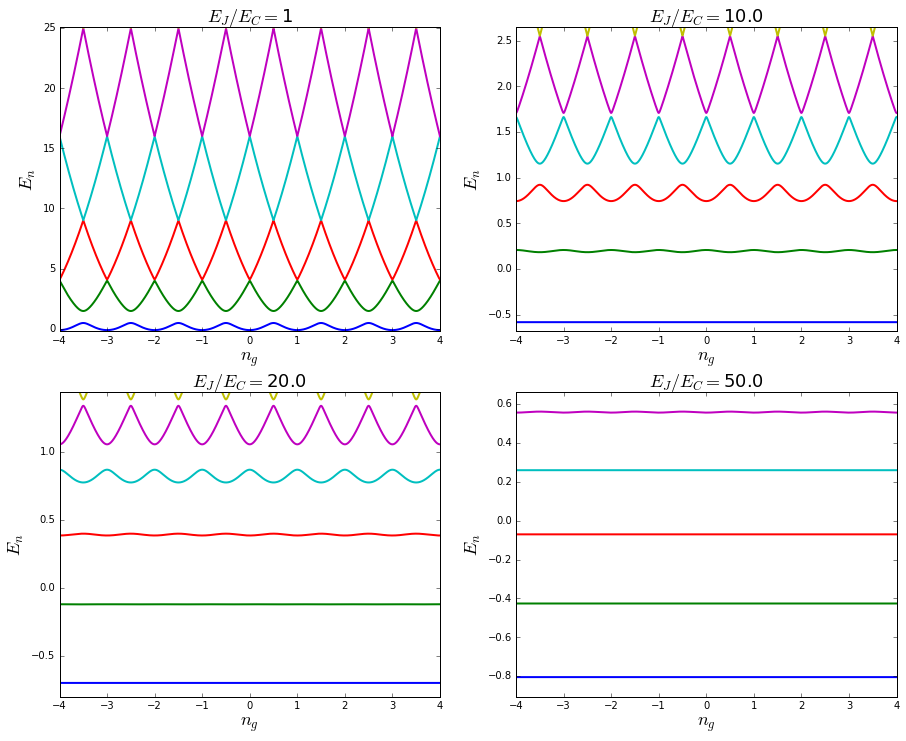
\includegraphics[width=\linewidth]{Figures/EjEcall.png}
\decoRule
\caption[Different $E_J/E_C$]{Energy levels for different $E_J/E_C$ values. Charge noise goes to zero as $E_J/E_C$ increases. Anharmonicity is also low but non-zero. This figure was generated using \cite{Johansson2012}.}
\label{fig:diff EJ/EC}
\end{figure}

As we can see the charge noise is very low for the case of high $E_J/E_C$. Also, anharmonicity, which is defined as $\alpha_h=E_{21}-E_{10}$, is reduced but not zero. In-fact, charge noise reduces exponentially while anharmonicity reduces only algebraically as $E_J/E_C$ is increased. This is the basis on which the transmon qubit is realised.

The Hamiltonian can also be solved using perturbation theory in the limit $E_J/E_C\gg 1$ by expanding the cosine in the tunnelling energy up to fourth order and treating the fourth order term as a perturbation. There is no dependence on $n_g$ because the system is charge insensitive at high $E_J/E_C$. The energy levels are \cite{Koch2007a}

\begin{equation}
E_k\approx-E_J+\sqrt{8E_CE_J}\left(k+\frac{1}{2}\right)-\frac{E_C}{12}(6k^2+6k+3)
\label{eqn:transmon levels}
\end{equation}

From \ref{eqn:transmon levels} we can see that the qubit transition frequency ($\omega_{10}$) is
\begin{equation}
\omega_{10}=\frac{E_1-E_0}{\hbar}=\frac{\sqrt{8E_JE_C}-E_C}{\hbar}
\end{equation}
and the anharmonicity
\begin{equation}
\alpha_h=(E_2-E_1)-(E_1-E_0)=-E_C
\end{equation}

\section{Coupling the Transmon to a Resonator}

For qubit readout and control, we will couple the qubit to a microwave cavity resonator (A rectangular waveguide resonator in this case). The lumped element circuit model of the qubit and cavity resonator is shown in Fig.\ref{fig:transmon with cavity}.

\begin{figure}
\centering
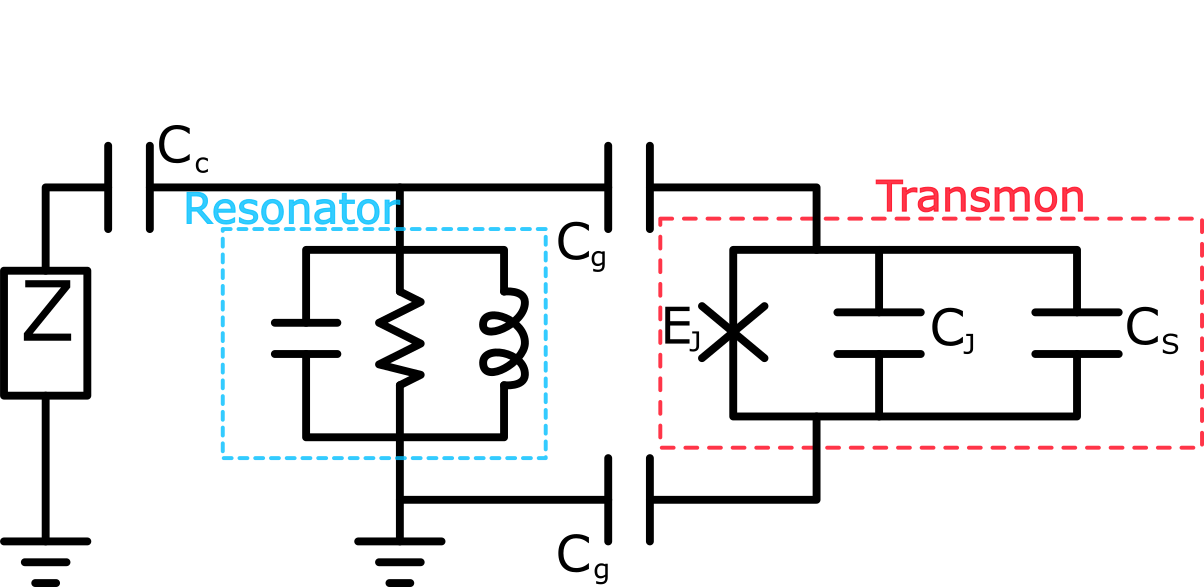
\includegraphics[width=\linewidth]{Figures/transmon_circuit.png}
\decoRule
\caption[Transmon Circuit]{Transmon coupled to the resonator coupled to the measurement device.}
\label{fig:transmon with cavity}
\end{figure}

We can approximate the transmon as a 2 level system with a ground state $\ket{g}$ and excited state $\ket{e}$ for large anharmonicity. In this approximation, the Hamiltonian of the system is discussed below  \cite{Richer2013,Schuster2007}.
\begin{itemize}
\item The Hamiltonian of the transmon can be expressed as the following if we choose the coordinate system appropriately and the zero energy as the mean energy of the transmon
\begin{equation}
\hat{\mathcal{H}}_{qubit}=-\frac{\hbar\omega_q}{2}\sigma_z
\label{eqn:qubit free hamiltonian}
\end{equation}
\item The Hamiltonian of the resonator is the same as the one for  an LC oscillator \ref{eqn:harmonic hamiltonian}
\begin{equation}
\hat{\mathcal{H}}_{cavity}=\hbar\omega_ra^\dag a
\end{equation}
The ground state energy of $\hbar\omega_r/2$ has not been shown as it does not have any significance in qubit dynamics.
\item The interaction hamiltonian is given by 
\begin{equation}
\hat{\mathcal{H}}_{int}=\hbar g(a^\dag\sigma_-+a\sigma_+)
\end{equation}
where $g$ is the coupling constant, proportional to the amplitude of the signal. The rotating wave approximation is made here, ignoring terms with $a^\dag\sigma_+$ and $a\sigma_-$.
\end{itemize}

This gives us the Jaynes-Cummings Hamiltonian
\begin{equation}
\hat{\mathcal{H}}=\hbar\omega_ra^\dag a-\frac{\hbar\omega_q}{2}\sigma_z+\hbar g(a^\dag\sigma_-+a\sigma_+)
\end{equation}

The eigenstates for the coupled system are
\begin{subequations}
\label{eqn:coupled eigenstates}
\begin{align}
\ket{n,+} &= \cos\frac{\theta_n}{2}\ket{e}\ket{n}+\sin\frac{\theta_n}{2}\ket{g}\ket{n+1}\\
\ket{n,-} &= -\sin\frac{\theta_n}{2}\ket{e}\ket{n}+\cos\frac{\theta_n}{2}\ket{g}\ket{n+1}
\end{align}
\end{subequations}
with eigenenergies
\begin{equation}
E_{n\pm}=\hbar\omega_r n\pm\frac{\sqrt{\hbar^2\Delta^2+4g^2(n+1)}}{2}
\end{equation}
where $\Delta=\omega_r-\omega_q$ and
\begin{equation}
\theta_n = \tan^{-1}\left(\frac{2g\sqrt{n+1}}{\hbar \Delta}\right)
\end{equation}

\section{The Bloch Sphere}

A general pure state for a two level system can represented as
\begin{equation}
\ket{\psi} = c_0\ket{0}+c_1\ket{1}
\end{equation}
where $\ket{0}$ and $\ket{1}$ form an orthonormal basis. $c_0=|c_0|e^{j\phi_1}$ and $c_1=|c_1|e^{j\phi_2}$ are complex numbers with a constraint that $|c_0|^2+|c_1|^2 = 1$ due to normalization. Since one can only measure the phase difference $\phi = \phi_2-\phi_1$, the state can be represented as
\begin{equation}
\ket{\psi} = \cos\frac{\theta}{2}\ket{0}+e^{j\phi}\sin\frac{\theta}{2}\ket{1}
\end{equation}
with no loss of generality where $\theta= 2\cos^{-1}|c_0|=2\sin^{-1}|c_1|$.

This state can be represented on a sphere with spherical coordinates on the surface with radius $r = 1$. The $\ket{0}$,$\ket{1}$ and an arbitrary state is shown in the Bloch Sphere in Fig.\ref{fig:bloch rep}.

\begin{figure}
\centering
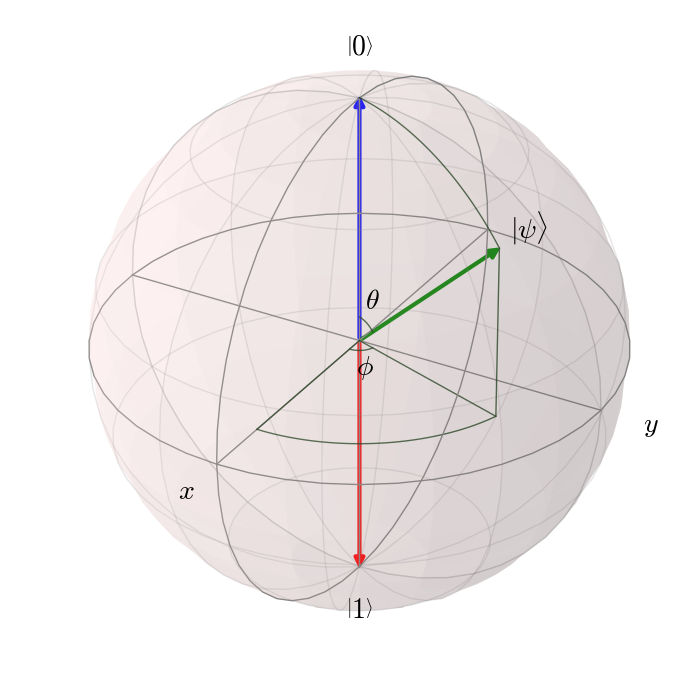
\includegraphics[width=\linewidth]{Figures/bloch_rep.png}
\decoRule
\caption[Bloch Sphere Representation]{Representation of states on a Bloch Sphere. The blue arrow represents the ground state $\ket{g}$, the red arrow represents the excited state $\ket{e}$, and the green arrow represents an arbitrary state $\ket{\psi} = \cos(\theta/2)\ket{g}+e^{j\phi}\sin(\theta/2)\ket{e}$.\\This figure was generated using \cite{Johansson2012}.}
\label{fig:bloch rep}
\end{figure}

\section{Dynamics of the Jaynes-Cummings system}

Let us consider the dynamics of the system in three different cases that are relevant to qubit manipulation and readout.
\begin{itemize}
\item \textbf{Zero Coupling} ($g=0$)\\
If there is no coupling (no photons in the cavity), then the qubit follows the free Hamiltonian given by \ref{eqn:qubit free hamiltonian}. The energy eigenstates of this system are $\ket{g}$ and $\ket{e}$ with energies $-\hbar\omega_q/2$ and $\hbar\omega_q/2$ respectively. In this basis, the Hamiltonian of the qubit can be expressed as
\begin{equation}
\hat{\mathcal{H}}_{qubit} = -\hbar\omega_q/2\ket{e}\bra{e} + \hbar\omega_q/2\ket{g}\bra{g}
\end{equation}
Applying the unitary operator $e^{i\hat{\mathcal{H}}t/\hbar}$ to an initial superposition state $\ket{\psi(0)}=c_0\ket{e}+c_1\ket{g}$ gives the state at a time $t$
\begin{align}
\begin{split}
\ket{\psi(t)} &= e^{i\hat{\mathcal{H}}t/\hbar}\ket{\psi(0)}\\
&=e^{-i\omega_qt/2}\left(c_0\ket{e}+e^{i\omega_q t}c_1{g}\right)
\end{split}
\end{align}

\begin{figure}
\centering
\begin{subfigure}[b]{0.45\textwidth}
\centering
\includegraphics[width=\textwidth]{Figures/rotatez.png}
%\decoRule
\caption{No Coupling}
\label{fig:rotatez}
\end{subfigure}
\hfill
\begin{subfigure}[b]{0.45\textwidth}
\centering
\includegraphics[width=\textwidth]{Figures/rotatex.png}
%\decoRule
\caption{On Resonance}
\label{fig:rotatex}
\end{subfigure}
\decoRule
\caption[Qubit Evolution on Bloch Sphere]{Evolution of an arbitrary state on the Bloch sphere. The light blue arrow represents the initial state and the dark blue arrow represents the final state. This figure was generated using \cite{Johansson2012}.}
\label{fig:rotatexz}
\end{figure}

We can see that if the qubit starts in an eigenstate, it remains in the same state (only a phase factor is added), but if it starts in a superposition, it's phase oscillates as a function of time with a frequency equal to the qubit frequency. On the bloch sphere this can be represented as a precession about the $z$-axis as shown in Fig.\ref{fig:rotatez}.

We can consider the dynamics of the coupled system in a similar way, once we change the basis to the new energy eigenstates in \ref{eqn:coupled eigenstates}.

\item \textbf{On Resonance} ($\Delta\ll g$)\\
If the drive signal or photons are at the same frequency as the qubit, then $\Delta=0$, which implies $\theta_n=\pi/2$. Then the eigenstates are
\begin{subequations}
\label{eqn:delta zero eigenstates}
\begin{align}
\ket{n,+} &= \frac{1}{\sqrt{2}}\ket{e}\ket{n}+\frac{1}{\sqrt{2}}\ket{g}\ket{n+1}\\
\ket{n,-} &= -\frac{1}{\sqrt{2}}\ket{e}\ket{n}+\frac{1}{\sqrt{2}}\ket{g}\ket{n+1}
\end{align}
\end{subequations}
With the new eigenstates, the qubit will oscillate about the $x$-axis as shown in Fig.\ref{fig:rotatex}. This means that if the initial state of the qubit is $\ket{g}$, it will oscillate to $\ket{e}$ in time $t=\pi g\sqrt{n+1}$. A pulsed signal which causes this transition\footnote{This signal refers to any signal which is resonant with the qubit and causes a rotation of $\pi$ radians about the $x$-axis on the Bloch Sphere.} is called a $\pi$-pulse The excitation number of the cavity will also oscillate from $\ket{n+1}$ to $\ket{n}$ with the same frequency.

It is worth noting that if the resonant frequency of the cavity is far from that of the qubit, and if the drive signal is of qubit frequency, then the qubit will still oscillate because it takes finite time for the photons to decay in the cavity.

\item \textbf{Low Power Dispersive limit} ($\Delta\gg g$)\\
In the low power dispersive limit\footnote{For the high power limit see \cite{Bishop2010}. The specific case of the transmon in the high power limit is discussed in \cite{Boissonneault2010}.}, the number of photons in the cavity is low ($\approx$ 1-100). We can rewrite the Hamiltonian by considering $g/\Delta$ as a perturbation since $\Delta\gg g$ \cite{Schuster2007} to get
\begin{equation}
\hat{\mathcal{H}}=\hbar\left(\omega_r+\frac{g^2}{\Delta}\sigma_z\right)a^\dag a+\frac{\hbar}{2}\left(\omega_q+\frac{g^2}{\Delta}\right)\sigma_z
\label{eqn:dispersive hamiltonian}
\end{equation}

\begin{figure}
\centering
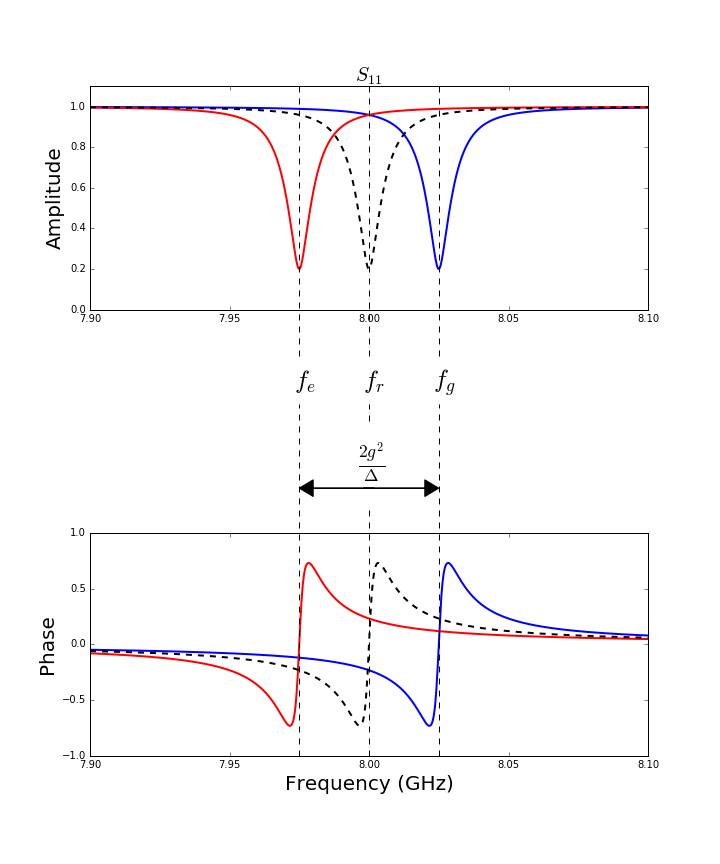
\includegraphics[width=\linewidth]{Figures/dispersive_shift.png}
\decoRule
\caption[Dispersive Shift]{Amplitude and Phase of $S_{11}$ for bare resonator (thick black dashed lines), resonator with qubit in ground state (thick blue line), and resonator with qubit in excited state (thick red line). The dispersive shift is $2g^2/\Delta$.}
\label{fig:dispersive shift}
\end{figure}

We can see from this Hamiltonian that dispersive coupling causes a shift of $\pm g^2/\Delta$ in the resonance frequency of the cavity depending on the qubit state. We can see the different $S_{11}$ parameter responses for the ground and excited states of the qubit in Fig.\ref{fig:dispersive shift}. This shift is crucial to measuring the state of the qubit.
We can also rearrange the equation as follows
\begin{equation}
\hat{\mathcal{H}}=\hbar\omega_r a^\dag a+\frac{\hbar}{2}\left(\omega_q+\frac{g^2}{\Delta}a^\dag a+\frac{g^2}{\Delta}\right)\sigma_z
\end{equation}
to see that the frequency of the qubit now has an added Lamb and ac-Stark shift of $g^2/\Delta$ and $g^2n/\Delta$ respectively \cite{Blais2004}.

The Hamiltonian in \ref{eqn:dispersive hamiltonian} can be written as
\begin{equation}
\hat{\mathcal{H}} = \hat{\mathcal{H}}_0 + \hat{\mathcal{H}}_{int}
\end{equation} 
where
\begin{equation}
\hat{\mathcal{H}}_0=\hbar\omega_r a^\dag a + \frac{\hbar\omega_q}{2} \sigma_z\
\end{equation}
is the uncoupled Hamiltonian of the qubit and cavity and
\begin{equation}
\hat{\mathcal{H}}_{int}=\frac{\hbar g^2\sigma_z}{\Delta}\left(a^\dag a+\frac{1}{2}\right)
\end{equation}
is the interaction Hamiltonian.\\

The unitary time evolution operator given by $\hat{U}(t)=e^{-j\hat{\mathcal{H}}t/\hbar}$ is
\begin{align}
\begin{split}
\hat{U}(t) = \text{exp}\left(-j\hat{\mathcal{H}}_0t/\hbar\right)\Bigg[&\text{ exp}\left(-j\frac{g^2t}{\Delta}\left(\hat{n}+\frac{1}{2}\right)\right)\ket{g}\bra{g}\\
+&\text{ exp}\left(j\frac{g^2t}{\Delta}\left(\hat{n}+\frac{1}{2}\right)\right)\ket{e}\bra{e}\Bigg]
\end{split}
\end{align}
If the initial state is such that the cavity is in a coherent state $\ket{\alpha}$ and the qubit is in a superposition state $(\ket{g}+\ket{e})/\sqrt{2}$, i.e
\begin{equation}
\ket{\psi(0)} = \frac{(\ket{g}+\ket{e})}{\sqrt{2}}\ket{\alpha}
\end{equation}
we can apply the unitary time evolution operator on this state and use the following relation
\begin{equation}
e^{i\varphi\hat{n}}\ket{\alpha} = \sum_{n=0}^\infty \frac{\alpha^ne^{i\varphi n}}{\sqrt{n!}}e^{-\frac{|\alpha|^2}{2}}\ket{n} = \ket{\alpha e^{i\varphi}}
\end{equation}
to get
\begin{align}
\begin{split}
\ket{\psi(t)} &= \hat{U}(t)\ket{\psi(0)}\\
&= \text{exp}\left(-j\hat{\mathcal{H}}_0t/\hbar\right)\frac{1}{\sqrt{2}}\Bigg[e^{-j\varphi/2}\ket{g}\ket{\alpha e^{-j\varphi}}+e^{j\varphi/2}\ket{e}\ket{\alpha e^{j\varphi}}\Bigg]
\end{split}
\end{align}
where $\varphi = g^2t/\Delta$. We can see that the cavity and qubit states are now entangled. The qubit ground state is entangled with the coherent state rotated by an angle $-\varphi$ and the excited state is entangled with the coherent state rotated by an angle $\varphi$.

At low powers, dispersive measurement is QND or Quantum Non-Demolition, which means that the qubit will remain in the eigenstate that was measured after a measurement. This means that repeated measurements will yield the same results.
\end{itemize}

\section{Decoherence}

A qubit which is initially in a superposition state $\ket{\psi} = \alpha\ket{g}+\beta\ket{e}$ will not stay in the superposition forever. It will lose its quantum information stochastically at a rate described below. The time for which the qubit retains its quantum information is called "coherence time", and is denoted by $T_2$. There are 2 processes which cause decoherence \cite{Geerlings2013}.
\begin{itemize}
\item \textbf{Relaxation}
The decay of the qubit to the ground state $\ket{g}$ due to spontaneous emission is referred to as relaxation. It does this at a rate $\Gamma_{\downarrow}$. If the qubit is in contact with a thermal bath at non zero temperature, there will also be excitation processes at a rate $\Gamma_{\uparrow}$. The combined effect gives the relaxation time $T_1 = \left(\Gamma_{\downarrow}+\Gamma_{\uparrow}\right)^{-1}$. Relaxation processes can be attributed to phenomena that cause energy fluctuations.
\item \textbf{Dephasing}
Dephasing is the process by which the qubit loses its phase information due to fluctuations is qubit frequency. These fluctuations cause the qubit to gain or lose phase and on average, lead to a diffused phase.
\end{itemize}

\section{Measurement Theory (Dispersive Limit)}

The setup for measurements is shown in Fig.\ref{fig:measurement setup}. All measurements described here assume that the cavity is dispersively coupled with the qubit. A signal of frequency $\omega_p$ is generated from port 1 of the VNA. This signal will be referred to as the probe signal. Another signal of frequency $\omega_d$ is combined with the probe signal and is sent into the cavity. This second signal is the drive signal. The VNA records the signal at port 2.

\begin{figure}
\centering
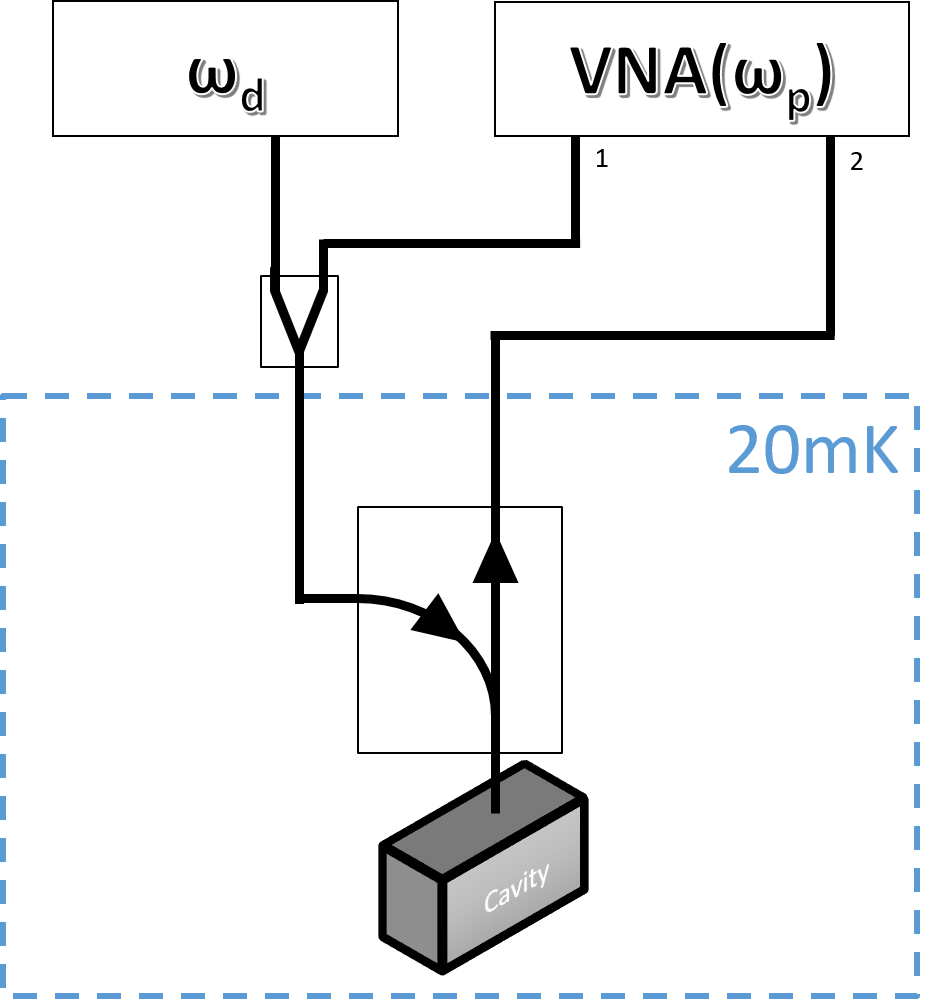
\includegraphics[width=400px]{Figures/measurement_circuit.png}
\decoRule
\caption[Measurement Setup]{Measurement Setup. The probe signal from the VNA and the drive signal from the signal generator is combined using a power combiner.}
\label{fig:measurement setup}
\end{figure}

\subsection{Single tone measurement}

In this measurement the drive signal is switched off and only the probe signal is sent to the cavity. We can plot the amplitude as a function of power and frequency of this signal. During this measurement, the qubit remains in the ground state except at high powers. This measurement was performed in \cite{Paik2011} with a 3D Transmon. The result of this measurement is similar to the ground state measurement in \cite{Reed2010}.

If the qubit is excited with a $\pi$-pulse at every point (i.e. for each frequency and power) and the amplitude is recorded for a certain period of time ($\approx$ 400 ns) and averaged, we can see the response of both the ground state and excited states. This experiment was performed in \cite{Reed2010} with a 2D Transmon.

\begin{itemize}
\item \textbf{Low Power Measurement}

The resonance occurs at the dispersively shifted frequency for low powers as expected.

\item \textbf{High Power Measurement}

At high powers, the resonance shifts toward the bare cavity frequency. This is described as a bright state of the cavity and is discussed in \cite{Bishop2010}. The specific case of the transmon is discussed in \cite{Boissonneault2010} where the transmon is treated as a Multi Level System.
\end{itemize}


\subsection{Two tone measurement}

Both the probe signal and drive signal are applied continuously in this measurement. The probe frequency is close to the cavity frequency and is used to populate the cavity with photons. The drive frequency is close to the qubit frequency and is used to manipulate the qubit. Application of the drive frequency exactly at the qubit frequency will cause the qubit to leave the ground state. If this drive tone is applied continuously, the qubit will have an equal probability of being in the ground and excited state, so there will be no dispersive shift.

Varying the frequencies and powers of the two signals can produce useful results.
\begin{itemize}
\item By probing the cavity with a fixed low power and a frequency equal to the cavity frequency, while varying the frequency of the drive signal at constant power, we can see a phase shift in the signal when the drive tone is at the qubit first transition frequency ($\omega_{01}$). For larger powers of the drive signal, the phase shift is larger. At sufficiently large powers, we can also see the qubit transition to the second excited level at $\omega_{12}$.
\item If the drive signal is swept at a constant power and the probe power is increased, we can see the qubit frequency changing as a result of ac-Stark shift as the number of photons in the cavity increase.
\item If the probe frequency is fixed close to the dispersively shifted resonance corresponding to one of the qubit states with a strong coupling rate and parameters such that $2\chi>\gamma,\kappa$, then spectroscopy with the drive frequency reveals the photon number state distribution in the cavity with different peaks corresponding to each photon number state. This is due to ac-Stark shift and is demonstrated using a \CPB in \cite{Schuster2007a}.
\end{itemize}

Details about Time Domain Measurements can be found in Appendix-\ref{AppendixB}